\subsection{La evolución de SOA: Microservicios}
\label{microservicios}

Como vimos en el apartado anterior, \gls{acro:soa} define qué principios debe cumplir un sistema distribuido para satisfacer los objetivos de la organización, que incluyen, facilidad y flexibilidad en la integración de sistemas \eng{legacy}, reducción en los costos de implementación y ágil adaptación a los cambios. Si bien esto ya establece precondiciones para un diseño, \gls{acro:soa} en sí no es un patrón concreto. Por el contrario, y similarmente a otros diseños de arquitectura de sistemas distribuidos como REST (el cual será tratado en la \autoref{standard:rest}), \gls{acro:soa} es un conjunto de propiedades que dichos sistemas debieran cumplir y a partir de los cuales podemos observar características comunes entre aquellos que sigan ese tipo de arquitecturas.

Es sobre la base de características de un tipo de sistemas como \gls{acro:soa} que se construyen luego los patrones de diseño. A modo de referencia se puede consultar el libro \eng{``SOA Patterns''} donde se definen más de 20 patrones orientados a servicios, como \eng{Service Host}\cite[p.~19]{soapatterns}, \eng{Composite Front End (Portal)}\cite[p.~148]{soapatterns} o \eng{Service Bus}\cite[p.162]{soapatterns}. Todos estos (y otros) patrones obedecen a los principios de las Arquitecturas Orientadas a Servicios, pero ninguno \textit{es} \gls{acro:soa} en sí mismo, ni \gls{acro:soa} \textit{es} solo uno de estos patrones. De hecho, si analizamos el caso particular de estos patrones podemos observar que inclusive pueden combinarse entre sí: el primero (\eng{Service Host}) guía en cómo se puede manejar el ambiente en que corren los servicios y los clientes de los mismos para simplificar su gestión, el segundo (\eng{Portal}) habla de cómo proveer una interfaz que combine más de un servicio, y el tercero (\eng{Service Bus}) propone la inclusión de un canal de comunicación previo a los servicios para gestionar las peticiones y respuestas con mejoras sobre la autogestión de peticiones por parte de los propios servicios.

En este contexto es que queremos centrarnos en un patrón de diseño de sistemas distribuidos emergente que se plantea como una alternativa al desarrollo de aplicaciones monolíticas.
Las aplicaciones monolíticas, típicamente consisten en componentes fuertemente acoplados, que son parte de una única unidad \eng{deployable}, resultando incómodo y dificultosa la incorporación de cambios, \eng{testing} y \eng{deployment} de la aplicación.  Es por esto que podemos encontrar ciclos de \eng{deployment} mensual (\eng{monthly deploymenbt}) en grandes organizaciones de IT.

El patrón de microservicios, trata estas cuestiones, separando la aplicación en múltiples unidades \eng{deployables} (\eng{service components}), que pueden ser desarrolladas, testeadas y deployadas independientemente de otros \eng{service component}. \todo{quizás tengamos que hablar mas de service component}.\cite[p.~27]{richards2015}

\begin{figure}
  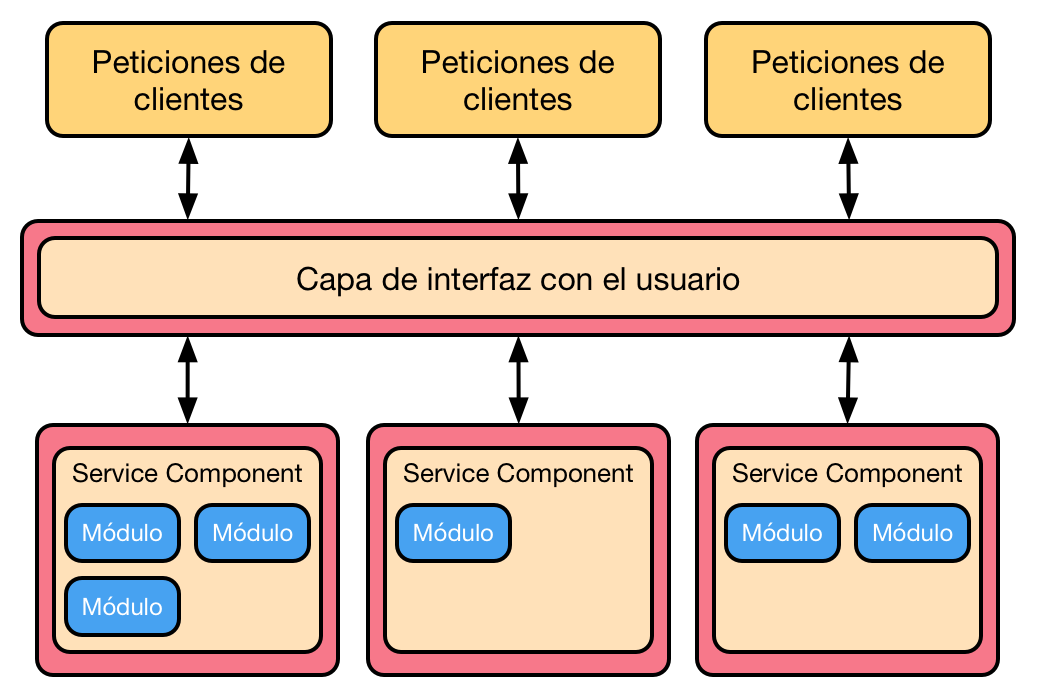
\includegraphics[width=\linewidth]{src/images/02-capitulo-2/basic_microservices_arquitecture_pattern.png}
  \caption{Arquitectura básica de microservicios}
  \label{fig:basic_microservices_arquitecture_pattern}
\end{figure}

Debido a que los componentes principales de una aplicación, se dividen en partes mas pequeñas, deployables de manera individual, las aplicaciones construídas utilizando el patrón de arquitectura de microservicios, son generalmente mas robustas, proporcionan una mejor escalabilidad y pueden soportar fácilmente ``continuous delivery'', permitiendo deployar en tiempo real en ambientes de producción, reduciendo significativamente la necesidad de deployments mensuales o semanales. \cite[p.~33]{richards2015} Todo esto es posible, dado que el cambio generalmente se encuentra aislado a un \eng{service component}, solo los \eng{service components} que cambian tienen que ser deployados.  Como se mencionó anteriormente, esta es una notable mejora frente al desarrollo de aplicaciones monolíticas, donde el fuerte acoplamiento en sus componentes, deriba en aplicaciones ``frágiles'' que se ``rompen'' o fallen con cada nuevo \eng{deployment}.

\todo{ver si se agrega la explicación de la diferentes topologías, o resumen nuestro}

Como se puede observar en \cite[p.~34]{richards2015}, se realiza un análisis de las siguientes características del patrón de arquitectura de microservicios:

\begin{itemize}

  \item El autor indica que este patrón, tiene un alto grado de \eng{overall agility}, que es la habilidad de responder rápidamente a los constantes cambios en el entorno.  Dado que es posible deployar unidades de forma separada, los cambios se encuentran aislados a \eng{service components} individuales, lo que permite \eng{deployments} sencillos y rápidos.
  Además, aplicaciones desarrolladas con este patrón, tienden a generarse con bajo acoplamiento, lo que ayuda en la incorporación de los cambios.

  \item \eng{Testability}
  Dado a la separación y aislamiento de las funcionalidad de negocio, el test de regresión para un \eng{service component} en particular, resulta más sencillo y factible, que un test de regresión realizado a toda una aplicación monolítica.  Además, dado que los \eng{service components} en este patrón están débilmente acoplados, hay menos posibilidades de que un desarrollador ``rompa'' la aplicación debido a la incorporación de un cambio reciente.

  \item Con respecto a la \eng{performance}, en general este patrón, debido a la naturaleza distribuida de la arquitectura de microservicios, no aporta en el desarrollo de aplicaciones de alto rendimiento.

  \item Desde el punto de vista de la \eng{scalability}, las aplicaciones se encuentran separadas en unidades deployables, cada \eng{service component} puede escalarse individualmente, permitiendo afinar la escalabilidad de acuerdo a las necesidades de la aplicación.

  \item \eng{Ease of development}
  Como la funcionalidad se encuentra separada en diferentes \eng{service components}, el desarrollo se vuelve mas sencillo, debido a un alcance mas pequeño y asilado.

\end{itemize}
